\chapter{Shift-left testing}\label{chapter:shift-left-testing}
In an article dated September 1st 2001 appeared in Dr. Dobb's Journal, Larry Smith wrote: 
\begin{quote}
\itshape
``Shift-left testing is how I refer to a better way of integrating the quality assurance (QA) and development parts of a software project.  By linking these two functions at lower levels of management, you can expand your testing program while reducing manpower and equipment needs - sometimes by as much as an order of magnitude.'' \cite{10.5555/500399.500404}
\end{quote}
This article is considered the manifesto of the shift-left movement, which is about moving the testing phase earlier in the software development lifecycle, shifting-left.

To give some background to the reader, up until the late 1990s, a typical software development process was sequential: the design was followed by the development, while testing and deployment were the latest phases of the project lifetime. Placing the testing phase at a late stage, bug fixing was costly and time-consuming. Sometimes developers had to even fully redesign the application in order to make everything behave correctly.
Kent Beck and Cynthia Andres wrote about this 
\begin{quote}
\itshape
``Here is the dilemma in software development: defects are expensive, but eliminating defects is also expensive. However, most defects end up costing more than it would have cost to prevent them.'' \cite{beck2004extreme}
\end{quote}

\begin{figure}[ht]
	\centering
	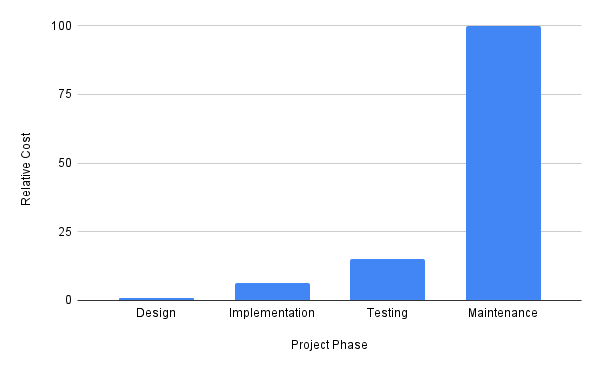
\includegraphics[width=1.0\textwidth]{Immagini/relative_cost_of_fixing_defects.jpg}
	\caption{Relative Cost of Fixing Defects}
	\label{fig:one}
\end{figure}

Listening to Larry Smith's suggestion, more and more teams try to integrate the quality assurance from the earlier phases of the development. The test-driven development is an approach that tries to do exactly this, designing the tests even before beginning the coding part. 
In addition, many tools were born to help the developers to ``shift-left'', like static analyzers. 
\\\\
It is important for the reader to understand that this kind of approach, aside from helping to find bugs early, thus reducing the costs implied by patches and code fixes, leads to a higher-quality product and codebase. This usually can help reduce the time to ship a product, avoiding unexpected issues and the need for refactoring existing parts of the code.
\\\\
In a software industry that is everyday more and more bound to other fields, especially safety-critical ones like medical, automobilistic and aeroespacial just to name a few, software quality is of the utmost importance, hence the \emph{``test early and often''} motto has become kind of a mantra for teams, which has now the instruments to catch defects as early as possible and in the least expensive way by integrating sane good practices and habits during the development.